\cleardoublepage%
\chapter{Theoretical Foundation}\label{ch:theoretical}
This chapter succinctly describes principles that build the foundation for later chapters.
Only the most relevant topics are touched upon, necessary details are explained in later chapters.
The mathematics that makes the techniques possible is not explained in-depth as it would otherwise
exceed the scope of this work.
Whenever possible heavy mathematical notation is omitted if it does not aid the reader's
understanding.

% XXX: note probabilistic view (distributions, frequentist/bayesian)
\section{Machine Learning}
A solid understanding of \ac{ML} has to be developed
first to grasp \ac{DL}~\citep{goodfellow_deep_2016}.
This is because \ac{DL} is a subfield of \ac{ML}~\citep{chauhan_review_2018}.
The most well-known definition for \ac{ML} comes from~\cite{mitchell_machine_1997}:
`A computer program is said to learn from experience $E$ with respect to some class of tasks $T$
and performance measure $P$, improves with experience $E$'.

% XXX: explain difference: model - algorithm
The task that the \ac{MLS} learns to perform can range from approximating a function
(e.g., regression --- $f:\R^n \rightarrow \R^l$, classification ---
$f:\R^n \rightarrow \{1,\ldots,k\}$) to obtaining a different representation for the data that
has beneficial properties for further processing but preserves as much information as possible
(e.g., PCA for compression)~\citep{goodfellow_deep_2016}.
Note that the learning itself is not the task but merely the process of improving on performing the
task~\citep{goodfellow_deep_2016}.
One of the most well-known \ac{ML} algorithms is Linear Regression.
In the following, the algorithm is used as an example for explaining \ac{ML} principles.
As the name implies, Linear Regression is used to predict a value $\hat{y}\in\R$ given the input vector
$\x\in\R^n$, which is made up of the features $x_i$.
The goal is to approximate the ground truth $y$.
Linear is derived from the underlying model shown in Equation~\ref{eq:linReg}:
\begin{equation}\label{eq:linReg}
    f(\x;\w,b) = \w^{T} \cdot \x + b = \sum_{i=1}^{n} w_i x_i + b = \hat{y}
\end{equation}
The scalar product of the weights $\w\in\R^n$ and \x\ is added to the bias term $b\in\R$.
Both $\w,b$ are parameters learned by the model to optimize the
approximation~\citep{goodfellow_deep_2016}.

The performance of a model measures how well the task can be completed.
Depending on the task of the \ac{MLS}, different quantitative measures are used.
The metric \ac{MSE} (see Equation~\ref{eq:mse}) can be used for Linear Regression.
\begin{equation}\label{eq:mse}
    \textsf{MSE} =\frac{1}{m}\norm{{(\hat{\textbf{y}} - \textbf{y})}}^2
        =\frac{1}{m}\sum_{i=1}^m {((\w^T \x^{(i)} + b) - \yti)}^2
\end{equation}
Here $m$ denotes the number of examples $\xti$ with the associated targets $\yti$, used to calculate
the error~\citep{geron_hands-machine_2017,goodfellow_deep_2016}.
The goal is to minimize the generalization error, which measures the expected performance on
previously unseen input~\citep{geron_hands-machine_2017}.
The test set is used once the model has been trained.
The test set is a part of the available data~\citep{geron_hands-machine_2017, goodfellow_deep_2016}.
The generalization error can be divided into three components.
The bias error arises from simplifying assumptions for the model; the variance error measures the
variation in the model outcome depending on the data used for training.
The model's representation capacity influences both these errors, so the
relationship is called the Bias/Variance tradeoff.
Lastly, the irreducible error stems from not having measured all data and the variation
in real data and cannot be
reduced~\citep{ashmore_assuring_2021, james_introduction_2013,geron_hands-machine_2017}.

The experience part of \ac{ML} depicts the process where the algorithm is `experiencing' the training
dataset $\Xt$ and is learning essential properties of the dataset.
In general, there are two paradigms for training: supervised and
unsupervised~\citep{goodfellow_deep_2016}.
Linear Regression is an example for supervised learning, as the model uses the ground truth value
to learn approximating $\yti$\ for the associated input
$\xti$~\citep{alzubi_machine_2018,goodfellow_deep_2016}.
For unsupervised learning, on the other hand, the algorithm is not directed to predict a target
value but to learn properties about the data and to leverage them for representation tasks
like compressing or denoising the data~\citep{goodfellow_deep_2016,geron_hands-machine_2017}.
In most cases, training can be described as an optimization problem, i.e., minimizing a
function --- the so-called objective or loss function $L$~\citep{goodfellow_deep_2016}.
The \ac{MSE} introduced earlier can be used for Linear Regression (see Equation~\ref{eq:mseOpt}).
This objective function has properties that make it suitable for linear output
models~\citep{goodfellow_deep_2016}.
\begin{equation}\label{eq:mseOpt}
    \min_{\w,b} \textsf{MSE}(\w,b)
\end{equation}
Note that for minimization, the \ac{MSE} is a function of $\w,b$, and not of $\x$.
In predicting a value, the \ac{MSE} is a function of $\x$ parametrized by $\w,b$ (see
Equation~\ref{eq:mseOpt}).
In Equation~\ref{eq:linReg} \w,$b$ are parameters that must be learned to minimize
the generalization error~\citep{james_introduction_2013,geron_hands-machine_2017}.
For other tasks such as binary classification, the metric (e.g., \fone) and the
objective function (binary cross entropy loss) are different~\citep{geron_hands-machine_2017,
ho_real-world-weight_2020}.
For optimization, the \ac{GD} algorithm is prevalent, especially in the subfield of \ac{DL}.
As the name suggests, the gradient is used to update the parameters $\w,b$ iteratively  to arrive
at a minimum of the objective function (see Equations~\ref{eq:gradDescW}
and~\ref{eq:gradDescb})~\citep{geron_hands-machine_2017}.
\begin{equation}\label{eq:gradDescW}
    \w'\leftarrow \w-\epsilon\cdot\nabla_{\w} \textsf{MSE}(\w,b)
        = \w-\frac{2\epsilon}{m}\Xt^T (\Xt\w+b-\y)
\end{equation}
\begin{equation}\label{eq:gradDescb}
    b'\leftarrow b-\epsilon\cdot\frac{\delta}{\delta b} \textsf{MSE}(\w,b)
        = b-\frac{2\epsilon}{m}(\Xt\w+b-\y)
\end{equation}

\begin{figure}[hb]
    \centering
    {\scriptsize%
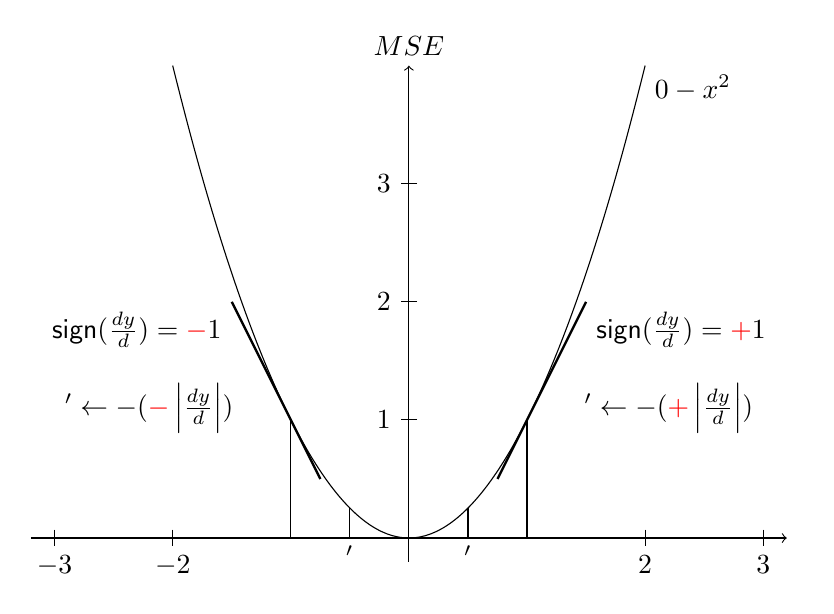
\begin{tikzpicture}[scale=1.5]
    \draw[->] (-3.2,0) -- (3.2,0) node[right] {$\w$};
    \draw[->] (0,-0.2) -- (0,4) node[above] {$MSE$};

    \foreach \x/\xtext in {2/2, 3/3}
        \draw[shift={(\x,0)}] (0pt,2pt) -- (0pt,-2pt) node[below] {$\xtext$};
    \foreach \x/\xtext in {-3/-3, -2/-2}
        \draw[shift={(\x,0)}] (0pt,2pt) -- (0pt,-2pt) node[below] {$\xtext$};
    \foreach \y/\ytext in {1/1, 2/2, 3/3}
        \draw[shift={(0,\y)}] (2pt,0pt) -- (-2pt,0pt) node[left] {$\ytext$};

    \draw (-2,4) parabola bend (0,0) (2,4) node[below right] {$\norm{0-x}^2$};
    \draw[-,line width=0.03cm] (0.75,0.5) -- (1.5,2) node[below right]
    {$\textsf{sign}(\frac{dy}{d\w})=\textcolor{red}{+}1$};
    \draw[-,line width=0.03cm] (-0.75,0.5) -- (-1.5,2) node[below left]
    {$\textsf{sign}(\frac{dy}{d\w})=\textcolor{red}{-}1$};

    \node at (2.2, 1.1) {$\w' \leftarrow \w - (\textcolor{red}{+}\left|\frac{dy}{d\w}\right|)$};
    \node at (-2.2, 1.1) {$\w' \leftarrow \w - (\textcolor{red}{-}\left|\frac{dy}{d\w}\right|)$};

    \draw[-] (1,1) -- (1,0);
    \draw[-] (-1,1) -- (-1,0);
    \draw[-] (0.5,0.25) -- (0.5,0);
    \draw[-] (-0.5,0.25) -- (-0.5,0);

    \node at (1, -0.2) {$\w$};
    \node at (-1, -0.2) {$\w$};

    \node at (0.5, -0.155) {$\w'$};
    \node at (-0.5, -0.155) {$\w'$};
\end{tikzpicture}
}

    \caption[Gradient descent visualization]{%
        Visualization for gradient descent for
        a 1-dimensional objective function~\citep{goodfellow_deep_2016}\label{fig:grad-desc}
    }
\end{figure}
The learning rate constant $\epsilon$ can be adjusted to speed up or slow down the `steps' which
can affect the convergence~\citep{goodfellow_deep_2016}.
More sophisticated variations of the \ac{GD} algorithm are more suited for practical
application (e.g., RMSProp, Adam)~\citep{geron_hands-machine_2017}.
Note that the process minimizes the test error with the test set $\Xt$.
The effect on the generalization error depends on model capacity, which is the space of functions
the model enables~\citep{goodfellow_deep_2016}.
Linear Regression has the capacity to fit data with a linear relationship between features and
ground truth.
If the underlying relationship is more complicated than that, the model can only underfit the data
(model bias)~\citep{goodfellow_deep_2016}.
Polynomial Regression has more capacity than Linear Regression, for example.
Say the actual relationship between features and ground truth now actually is linear;
the Polynomial Regression model can overfit for statistical outliers in the training set, which is why
in this case, the model with the lower capacity can achieve a lower generalization
error~\citep{geron_hands-machine_2017}.
Therefore, it is essential to improve the bias/variance tradeoff.
Aside from model selection, different techniques are used to prevent overfitting
(Regularization)~\citep{goodfellow_deep_2016}.
\begin{figure}[h]
    \centering
    \subfigure[Linear Regression underfit\label{fig:lin-reg-under}]{%
        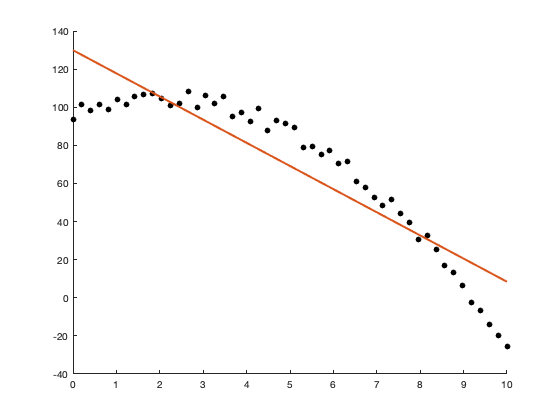
\includegraphics[width=0.45\textwidth]{img/Linear-Regression-underfit.png}
    }
    \subfigure[Polynomial Regression overfit\label{fig:pol-reg-over}]{%
        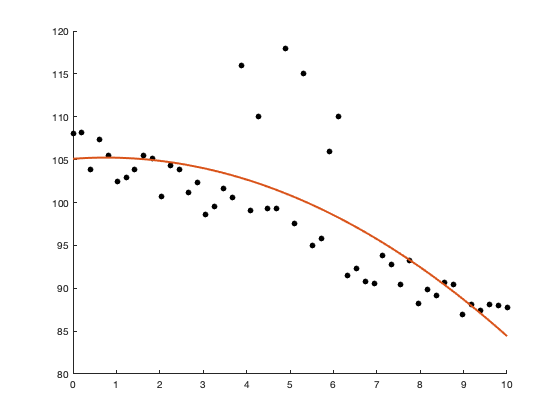
\includegraphics[width=0.45\textwidth]{img/Poly-Regression-overfit.png}
    }
    \caption[Regression over- and underfitting]{%
        Regression with linear and polynomial model\label{fig:examples}
    }
\end{figure}

\section{Deep Learning}
In \ac{DL}, \acp{DNN} are leveraged to learn new data representations through
multiple layers of abstraction automatically .
This makes \acp{DNN} powerful function approximators~\citep{goodfellow_deep_2016}.
\ac{DL} has only caught on in recent years as the enormous computational cost has been met
by improvement in computer hardware and automatic feature
learning~\citep{ponti_everything_2017, chen_text_2021}.
In this section, the basics of \acp{NN} are explained, and popular basic architectures thereof are
introduced.
% XXX: add freeing of researchers from manually crafting features \cite{long_scene_2021}

The most basic \ac{NN} is called a feedforward \ac{NN} or \ac{MLP}, where the information only
flows in one direction (in contrast to \acp{RNN} or Transformers)~\citep{goodfellow_deep_2016}.
The network is made up of so-called artificial neurons.
These neurons are arranged as a directed acyclic graph in multiple
layers~\citep{goodfellow_deep_2016}.
The first layer, which receives the input features $\x$, is called the input layer, the last layer
which outputs the final estimation of $\hat{y}$ or $\hat{\y}$ is called the output layer, all layers in between
are called the hidden layers~\citep{shrestha_review_2019}.
The structure with which the \ac{NN} is built in terms of how many layers, how many neurons are in
each layer, and how they are connected, is called architecture~\citep{goodfellow_deep_2016}.
The number of layers $d$ is referred to as depths, whereas the dimensionality of those layers is
called the width $w$~\citep{goodfellow_deep_2016}.
\begin{figure}[ht]
	\centering
    \begin{figure}[ht]
	\centering
	\begin{tikzpicture}[shorten >=1pt]
		\tikzstyle{unit}=[draw,shape=circle,minimum size=1.15cm]
		\tikzstyle{hidden}=[draw,shape=circle,minimum size=1.15cm]

		\node[unit](x0) at (0,3.5){$x_0$};
		\node[unit](x1) at (0,2){$x_1$};
		\node at (0,1){\vdots};
		\node[unit](xd) at (0,0){$x_D$};

		\node[hidden](h10) at (3,4){$z_0^{(1)}$};
		\node[hidden](h11) at (3,2.5){$z_1^{(1)}$};
		\node at (3,1.5){\vdots};
		\node[hidden](h1m) at (3,-0.5){$z_{m^{(1)}}^{(1)}$};

		\node(h22) at (5,0){};
		\node(h21) at (5,2){};
		\node(h20) at (5,4){};

		\node(d3) at (6,0){$\ldots$};
		\node(d2) at (6,2){$\ldots$};
		\node(d1) at (6,4){$\ldots$};

		\node(hL12) at (7,0){};
		\node(hL11) at (7,2){};
		\node(hL10) at (7,4){};

		\node[hidden](hL0) at (9,4){$z_0^{(L)}$};
		\node[hidden](hL1) at (9,2.5){$z_1^{(L)}$};
		\node at (9,1.5){\vdots};
		\node[hidden](hLm) at (9,-0.5){$z_{m^{(L)}}^{(L)}$};

        \node[unit](y1) at (12,4){$\hat{y}_1^{(L+1)}$};
        \node[unit](y2) at (12,2.2){$\hat{y}_2^{(L+1)}$};
		\node at (12,1.2){\vdots};
        \node[unit](yc) at (12,0){$\hat{y}_C^{(L+1)}$};

		\draw[->] (x0) -- (h11);
		\draw[->] (x0) -- (h1m);

		\draw[->] (x1) -- (h11);
		\draw[->] (x1) -- (h1m);

		\draw[->] (xd) -- (h11);
		\draw[->] (xd) -- (h1m);

		\draw[->] (hL0) -- (y1);
		\draw[->] (hL0) -- (yc);
		\draw[->] (hL0) -- (y2);

		\draw[->] (hL1) -- (y1);
		\draw[->] (hL1) -- (yc);
		\draw[->] (hL1) -- (y2);

		\draw[->] (hLm) -- (y1);
		\draw[->] (hLm) -- (y2);
		\draw[->] (hLm) -- (yc);

		\draw[->,path fading=east] (h10) -- (h21);
		\draw[->,path fading=east] (h10) -- (h22);

		\draw[->,path fading=east] (h11) -- (h21);
		\draw[->,path fading=east] (h11) -- (h22);

		\draw[->,path fading=east] (h1m) -- (h21);
		\draw[->,path fading=east] (h1m) -- (h22);

		\draw[->,path fading=west] (hL10) -- (hL1);
		\draw[->,path fading=west] (hL11) -- (hL1);
		\draw[->,path fading=west] (hL12) -- (hL1);

		\draw[->,path fading=west] (hL10) -- (hLm);
		\draw[->,path fading=west] (hL11) -- (hLm);
		\draw[->,path fading=west] (hL12) -- (hLm);

		\draw [
            decorate,decoration={brace,amplitude=10pt},xshift=-4pt,yshift=0pt
        ] (-0.5,4) -- (0.75,4) node [black,midway,yshift=+0.6cm]{input layer};
		\draw [
            decorate,decoration={brace,amplitude=10pt},xshift=-4pt,yshift=0pt
        ] (2.5,4.5) -- (3.75,4.5) node [black,midway,yshift=+0.6cm]{$1^{\text{st}}$ hidden layer};
		\draw [
            decorate,decoration={brace,amplitude=10pt},xshift=-4pt,yshift=0pt
        ] (8.5,4.5) -- (9.75,4.5) node [black,midway,yshift=+0.6cm]{$L^{\text{th}}$ hidden layer};
		\draw [
            decorate,decoration={brace,amplitude=10pt},xshift=-4pt,yshift=0pt
        ] (11.5,4.7) -- (12.75,4.7) node [black,midway,yshift=+0.6cm]{output layer};
	\end{tikzpicture}
	\caption[Network graph for a MLP.]{
        Network graph of a $(L+1)$-layer perceptron with $D$ input units and $C$ output units.
        The $l^{\text{th}}$ hidden layer contains $m^{(l)}$ hidden units.
    }
	\label{fig:multilayer-perceptron}
\end{figure}

	\caption[Network graph for a MLP]{%
        Network graph of a $(L+1)$-layer perceptron with $D$ input units and $C$ output units.
        The $l^{\text{th}}$ hidden layer contains $m^{(l)}$ hidden
        units~\citep{chauhan_review_2018,goodfellow_deep_2016}.\label{fig:multilayer-perceptron}
    }
\end{figure}
A neuron, the basic building block of \acp{NN}, receives input from neurons in the previous layer
and calculates a single value propagated to neurons in the following
layer~\citep{shrestha_review_2019}.
The value is calculated by feeding the received information into a Linear Regression model (see
Equation~\ref{eq:linReg}).
The resulting value is fed into an activation function $g$ which introduces nonlinearity to allow
more complicated transformations of information and representation~\citep{goodfellow_deep_2016}.
\begin{equation}\label{eq:neuron}
    f(\x;\T) = g(\T\x)=\z
\end{equation}
Here $f$ denotes the function performed by a layer of neurons (linearity + activation).
The parameters of the individual neurons are grouped to $\T$ ($\T_{:,0}$ equals 1 for the
bias term).
Popular activation functions include \relu, \tahn, sigmoid ($\sigma$), and
\sfmx~\citep{shrestha_review_2019}.
\begin{equation}\label{eq:relu}
    \relu(x)=\max(0,x)
\end{equation}
\begin{equation}\label{eq:tanh}
    \tahn(x)=\frac{\exp(x)-\exp(-x)}{\exp{x}+\exp{-x}}
\end{equation}
\begin{equation}\label{eq:sigmoid}
    \sigma(x)=\frac{1}{1+\exp(-x)}
\end{equation}
\begin{equation}\label{eq:softmax}
    {\sfmx(\x)}_i = \frac{\exp(x_i)}{\sum_j \exp(x_j)}
\end{equation}
While \relu\ is the prevalent function for feedforward \ac{NN}~\citep{goodfellow_deep_2016},
$\tahn$ is often used in \acp{RNN} like in~\cite{sherstinsky_fundamentals_2020,greff_lstm_2017}.
Sigmoid (\sfmx) activation functions, used for the output layer, are used to generate a Bernoulli
(Multinouli) distribution which is helpful for classification tasks~\citep{goodfellow_deep_2016}.
For, e.g.\ regression, the output layer can omit the activation
function~\citep{goodfellow_deep_2016}.
The prediction calculation is a concatenation of the functions defined by the
layers and their neurons, the process of which is called
forward propagation~\citep{ponti_everything_2017,goodfellow_deep_2016}.
\begin{equation}\label{eq:NNconcat}
    \hat{y}=f(\ldots f(f(\x;\T^{(1)});\T^{(2)})\ldots;\T^{(d)})
\end{equation}
$\T^{(i)}$ in Equation~\ref{eq:NNconcat} stands for the parameters in layer i with $\T^{(i)}_{j,:}$
being the parameters the $j$-th neuron in that layer~\citep{goodfellow_deep_2016}.
The forward propagation can also be described by a computational graph (see
Figure~\ref{fig:multilayer-perceptron})~\citep{goodfellow_deep_2016}.

The term \ac{DNN} comes from adding many hidden layers to the \ac{NN}~\citep{shrestha_review_2019}.
This allows for a more complicated function and better-developed features or representations that
are extracted from the input feature vector $\x$~\citep{oyedotun_deep_2015}.
The \ac{DNN} can be trained as a whole, thus making feature engineering redundant in contrast to
standard \ac{ML} algorithms~\citep{arpteg_software_2018}.
The training algorithm is called backpropagation.
The training error is calculated through the objective function and is propagated
in conjunction with the output of forward propagation on each neuron~\citep{goodfellow_deep_2016}.
For this, the chain rule of calculus can be used to modularly recursively propagate the
loss backward to use \ac{GD} (see Figure~\ref{fig:error-backpropagation}).
% XXX: NNs are not convex
\begin{figure}[ht]
	\centering
    \begin{figure}[ht]
	\centering
	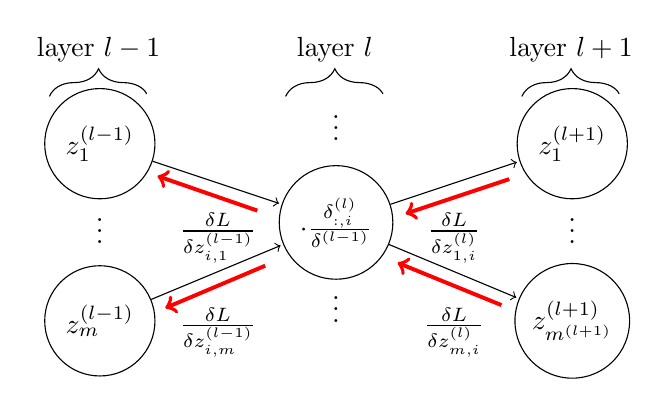
\begin{tikzpicture}[shorten >=1pt]
        \tikzstyle{unit}=[draw,shape=circle,minimum size =1.4cm]


		\draw [
            decorate,decoration={brace,amplitude=10pt},xshift=-4pt,yshift=0pt
        ] (-0.5,2.6) -- (0.75,2.6) node [black,midway,yshift=+0.6cm]{layer $l-1$};
        \node[unit](p1) at (0,2){$z_1^{(l-1)}$};
		\node at (0, 1){$\vdots$};
        \node[unit](pm) at (0,-0.25){$z_{m}^{(l-1)}$};

		\draw [
            decorate,decoration={brace,amplitude=10pt},xshift=-4pt,yshift=0pt
        ] (2.5,2.6) -- (3.75,2.6) node [black,midway,yshift=+0.6cm]{layer $l$};
		\node at (3, 2.3){$\vdots$};
        \node[unit](i) at (3,1){$\cdot\frac{\delta \z_{:,i}^{(l)}}{\delta \z^{(l-1)}}$};
		\node at (3, 0){$\vdots$};

		\draw [
            decorate,decoration={brace,amplitude=10pt},xshift=-4pt,yshift=0pt
        ] (5.5,2.6) -- (6.75,2.6) node [black,midway,yshift=+0.6cm]{layer $l+1$};
        \node[unit](k1) at (6,2){$z_1^{(l+1)}$};
		\node at (6, 1){$\vdots$};
		\node[unit](km) at (6,-0.25){$z_{m^{(l+1)}}^{(l+1)}$};

        \draw[->] (p1) -- (i);
        \draw[->] (pm) -- (i);

        \draw[->] (i) -- (k1);
		\draw[->] (i) -- (km);

        \node at (1.5,0.8){$\frac{\delta L}{\delta z_{i,1}^{(l-1)}}$};
        \node at (1.5,-0.4){$\frac{\delta L}{\delta z_{i,m}^{(l-1)}}$};

		\draw[->,red,line width=0.05cm] (2.1,0.45) -- (0.8,-0.1);
		\draw[->,red,line width=0.05cm] (2,1.15) -- (0.7,1.6);

        \node at (4.5,0.8){$\frac{\delta L}{\delta z_{1,i}^{(l)}}$};
        \node at (4.5,-0.4){$\frac{\delta L}{\delta z_{m,i}^{(l)}}$};

		\draw[->,red,line width=0.05cm] (5.1,-0.05) -- (3.75,0.5);
		\draw[->,red,line width=0.05cm] (5.2,1.55) -- (3.85,1.1);

    \end{tikzpicture}

	\caption[Backpropagation of errors through the network.]{
        Reverse traversing the network's computation graph,
        $\cdot \frac{\delta z_{:,i}^{(l)}}{\delta \w_i^{(l)}}$ is used for
        updating.\label{fig:error-backpropagation}
    }
\end{figure}

	\caption[Backpropagation of errors through the network.]{%
        Reverse traversing the network's computation graph,
        $\cdot \frac{\delta \z_{:,i}^{(l)}}{\delta \w_i^{(l)}}$ is used for
        updating the neurons parameters with gradient descent\label{fig:error-backpropagation}
    }
\end{figure}
The upstream gradient coming from neurons in the next layer is multiplied with the
jacobian matrix of the current neuron to produce the downstream gradient that is then used by
the preceding layer~\citep{boue_deep_2018,goodfellow_deep_2016}.
\begin{equation}\label{eq:backPropNeuronW}
    \frac{\delta L}{\delta\w} = \frac{\delta L}{\delta\z} \frac{\delta\z}{\delta\w}
\end{equation}
\begin{equation}\label{eq:backPropNeuronX}
    \frac{\delta L}{\delta\x} = \frac{\delta L}{\delta\z}\frac{\delta\z}{\delta\x}
\end{equation}
The result of Equation~\ref{eq:backPropNeuronW} is used to update the neuron's weights \w\ while
the result of Equation~\ref{eq:backPropNeuronX} is used for further
propagation~\citep{boue_deep_2018}.
This calculation is performed until the first layer of the computational graph is
reached~\citep{goodfellow_deep_2016}.
Note that the algorithm can be performed with tensors of arbitrary
dimensionality~\citep{goodfellow_deep_2016}.

\section{Convoluational Neural Nets}\label{se:cnn}
% basics
\acp{CNN} are a type of \ac{NN} that is also acyclic or feedforward, like
\acp{MLP}~\citep{chauhan_review_2018}.
\acp{CNN} are specialized to process a grid of values $\X$ like an image~\citep{goodfellow_deep_2016}.
\acp{CNN} are extensively used in computer vision~\citep{chauhan_review_2018}.
They consist of a variety of components: fully connected layer, activation function,
convolutional layer, pooling layer~\citep{chauhan_review_2018,ponti_everything_2017}.
The fully connected layers are the layers that make up \acp{MLP}~\citep{ponti_everything_2017}.

% conv layer
A convolutional layer has multiple filters, which consist of multiple
kernels~\citep{chauhan_review_2018}.
For multi-layer input, with $d$ so-called channels, a filter has the same amount of kernels as there
are channels ($d$)~\citep{ponti_everything_2017}.
Note that the height and width are spatial dimensions, and the depth is referred to
as the channel dimension.
\begin{figure}[ht]
    \centering
    \begin{tikzpicture}[scale=0.1]
	\matrix (mtr) [matrix of nodes,row sep=-\pgflinewidth, nodes={draw}]
	{
		0 & 1 & 1 & |[fill=red!30]| 1 & |[fill=red!30]| 0 & |[fill=red!30]| 0 & 0\\
		0 & 0 & 1 & |[fill=red!30]| 1 & |[fill=red!30]| 1 & |[fill=red!30]| 0 & 0\\
		0 & 0 & 0 & |[fill=red!30]| 1 & |[fill=red!30]| 1 & |[fill=red!30]| 1 & 0\\
		0 & 0 & 0 & 1 & 1 & 0 & 0\\
		0 & 0 & 1 & 1 & 0 & 0 & 0\\
		0 & 1 & 1 & 0 & 0 & 0 & 0\\
		1 & 1 & 0 & 0 & 0 & 0 & 0\\
	};

	\draw[very thick, red] (mtr-1-4.north west) rectangle (mtr-3-6.south east);

	\node [below= of mtr-5-4.south] (lm) {Input};

	\node[right = 0.2em of mtr] (str) {$*$};

	\matrix (K) [right=0.2em of str,matrix of nodes,row sep=-\pgflinewidth, nodes={draw, fill=blue!30}]
	{
		1 & 0 & 1 \\
		0 & 1 & 0 \\
		1 & 0 & 1 \\
	};
	\node [below = of K-3-2.south] (lk) {Kernel};

	\node [right = 0.2em of K] (eq) {$=$};

	\matrix (ret) [right=0.2em of eq,matrix of nodes,row sep=-\pgflinewidth, nodes={draw}]
	{
		1 & 4 & 3 & |[fill=green!30]| 4 & 1\\
		1 & 2 & 4 & 3 & 3\\
		1 & 2 & 3 & 4 & 1\\
		1 & 3 & 3 & 1 & 1\\
		3 & 3 & 1 & 1 & 0\\
	};
	\node [below = of ret-4-3.south] (lim) {Feature map};

	\draw[very thick, green] (ret-1-4.north west) rectangle (ret-1-4.south east);

	\draw[densely dotted, blue, thick] (mtr-1-4.north west) -- (K-1-1.north west);
	\draw[densely dotted, blue, thick] (mtr-3-4.south west) -- (K-3-1.south west);
	\draw[densely dotted, blue, thick] (mtr-1-6.north east) -- (K-1-3.north east);
	\draw[densely dotted, blue, thick] (mtr-3-6.south east) -- (K-3-3.south east);

	\draw[densely dotted, green, thick] (ret-1-4.north west) -- (K-1-1.north west);
	\draw[densely dotted, green, thick] (ret-1-4.south west) -- (K-3-1.south west);
	\draw[densely dotted, green, thick] (ret-1-4.north east) -- (K-1-3.north east);
	\draw[densely dotted, green, thick] (ret-1-4.south east) -- (K-3-3.south east);

	\matrix (K) [right=0.2em of str,matrix of nodes,row sep=-\pgflinewidth, nodes={draw, fill=blue!10}]
	{
		1 & 0 & 1 \\
		0 & 1 & 0 \\
		1 & 0 & 1 \\
	};

	\draw[very thick, blue] (K-1-1.north west) rectangle (K-3-3.south east);

	\node[anchor=south east, inner sep=0.01em, blue] at (mtr-1-4.south east) (xx) {\scalebox{.5}{$\times 1$}};
	\node[anchor=south east, inner sep=0.01em, blue] at (mtr-1-5.south east) (xx) {\scalebox{.5}{$\times 0$}};
	\node[anchor=south east, inner sep=0.01em, blue] at (mtr-1-6.south east) (xx) {\scalebox{.5}{$\times 1$}};
	\node[anchor=south east, inner sep=0.01em, blue] at (mtr-2-4.south east) (xx) {\scalebox{.5}{$\times 0$}};
	\node[anchor=south east, inner sep=0.01em, blue] at (mtr-2-5.south east) (xx) {\scalebox{.5}{$\times 1$}};
	\node[anchor=south east, inner sep=0.01em, blue] at (mtr-2-6.south east) (xx) {\scalebox{.5}{$\times 0$}};
	\node[anchor=south east, inner sep=0.01em, blue] at (mtr-3-4.south east) (xx) {\scalebox{.5}{$\times 1$}};
	\node[anchor=south east, inner sep=0.01em, blue] at (mtr-3-5.south east) (xx) {\scalebox{.5}{$\times 0$}};
	\node[anchor=south east, inner sep=0.01em, blue] at (mtr-3-6.south east) (xx) {\scalebox{.5}{$\times 1$}};

\end{tikzpicture}

    \caption[Visualization of a convolution operation]{%
        Convolution operation of a single kernel~\citep{chauhan_review_2018}\label{fig:conv-layer}
    }
\end{figure}
A kernel is a $n\times n$ square matrix of learnable parameters, so a filter is a tensor
$n\times n\times d$.
The convolution operation is the elementwise multiplication between the filter and the input's
overlapping $n\times n$ subspace (see Figure~\ref{fig:conv-layer})~\citep{ponti_everything_2017}.
The convolution operation is performed for every space in the input.
Spaces can be skipped if stride is introduced~\citep{ponti_everything_2017}.
Often zero-padding is used to preserve the spatial dimensions between input and output of
the layer (known as same-padding)~\citep{ponti_everything_2017,simonyan_very_2015}.
The number of filters a convolutional layer applies is equal to the output channels that the layer
has, which are often called feature maps~\citep{ponti_everything_2017}.
The convolution result is usually fed into a \relu\ activation function to introduce
nonlinearity like with fully connected layers.
The activation is performed on every element in the output and preserves the
dimensionality~\citep{ponti_everything_2017}.
In the explained scenario, the filter is slid across a 2d-surface to perform convolution.
Note that this can be restricted to 1d (e.g., audio) or extended to 3d (e.g., CT
scans)~\citep{goodfellow_deep_2016}.

% pooling
\begin{figure}[h]
    \centering
    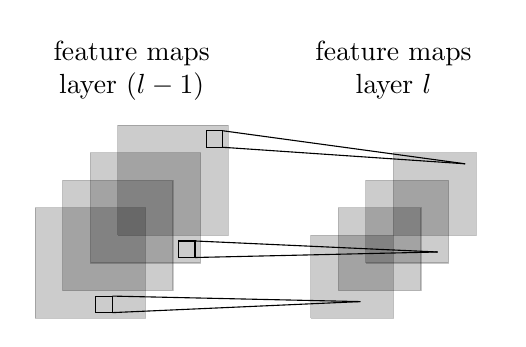
\begin{tikzpicture}[scale=0.7]
    \node at (1.75,4.5){\begin{tabular}{c}feature maps\\layer $(l-1)$\end{tabular}};

    \draw[fill=black,opacity=0.2,draw=black] (1.5,1.5) -- (3.5,1.5) -- (3.5,3.5) -- (1.5,3.5) -- (1.5,1.5);
    \draw[fill=black,opacity=0.2,draw=black] (1,1) -- (3,1) -- (3,3) -- (1,3) -- (1,1);
    \draw[fill=black,opacity=0.2,draw=black] (0.5,0.5) -- (2.5,0.5) -- (2.5,2.5) -- (0.5,2.5) -- (0.5,0.5);
    \draw[fill=black,opacity=0.2,draw=black] (0,0) -- (2,0) -- (2,2) -- (0,2) -- (0,0);

    \draw (3.1,3.1) -- (3.4,3.1) -- (3.4,3.4) -- (3.1,3.4) -- (3.1,3.1);
    \draw (2.6,1.1) -- (2.9,1.1) -- (2.9,1.4) -- (2.6,1.4) -- (2.6,1.1);
    \draw (1.1,0.1) -- (1.4,0.1) -- (1.4,0.4) -- (1.1,0.4) -- (1.1,0.1);

    \draw (3.4,3.4) -- (7.8,2.8);
    \draw (3.4,3.1) -- (7.8,2.8);

    \draw (2.9,1.4) -- (7.3,1.2);
    \draw (2.9,1.1) -- (7.3,1.2);

    \draw (1.4,0.4) -- (5.9,0.3);
    \draw (1.4,0.1) -- (5.9,0.3);

    \node at (6.5,4.5){\begin{tabular}{c}feature maps\\layer $l$\end{tabular}};

    \draw[fill=black,opacity=0.2,draw=black] (6.5,1.5) -- (8,1.5) -- (8,3) -- (6.5,3) -- (6.5,1.5);
    \draw[fill=black,opacity=0.2,draw=black] (6,1) -- (7.5,1) -- (7.5,2.5) -- (6,2.5) -- (6,1);
    \draw[fill=black,opacity=0.2,draw=black] (5.5,0.5) -- (7,0.5) -- (7,2) -- (5.5,2) -- (5.5,0.5);
    \draw[fill=black,opacity=0.2,draw=black] (5,0) -- (6.5,0) -- (6.5,1.5) -- (5,1.5) -- (5,0);
\end{tikzpicture}
%
    \caption[Channel dimension preserving of pooling layers]{%
        Pooling layers preserve channel dimenstions but downsample spatial
        dimensions\label{fig:pool-layer}
    }
\end{figure}
Pooling layers are used to reduce the spatial dimension (i.e., downsampling) of feature
maps~\citep{ponti_everything_2017}.
Pooling layers preserve the number of channels, as the operation is performed to each channel
separately (see Figure~\ref{fig:pool-layer})~\citep{chauhan_review_2018}.
\begin{figure}[ht]
    \centering
    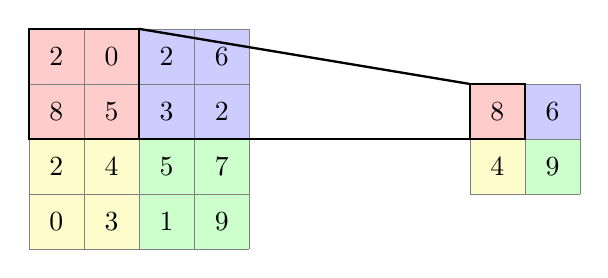
\begin{tikzpicture}[scale=0.7]
    \fill[yellow!20] (0,0) rectangle (2,2);
    \fill[red!20] (0,2) rectangle (2,4);
    \fill[green!20] (2,0) rectangle (4,2);
    \fill[blue!20] (2,2) rectangle (4,4);

    \draw[gray,very thin] (0,0) grid (4,4);

    \node at (0.5,0.5) {0};
    \node at (1.5,0.5) {3};
    \node at (0.5,1.5) {2};
    \node at (1.5,1.5) {4};

    \node at (2.5,0.5) {1};
    \node at (3.5,0.5) {9};
    \node at (2.5,1.5) {5};
    \node at (3.5,1.5) {7};

    \node at (0.5,2.5) {8};
    \node at (1.5,2.5) {5};
    \node at (0.5,3.5) {2};
    \node at (1.5,3.5) {0};

    \node at (2.5,2.5) {3};
    \node at (3.5,2.5) {2};
    \node at (2.5,3.5) {2};
    \node at (3.5,3.5) {6};

    \fill[yellow!20] (8,1) rectangle (9,2);
    \fill[red!20] (8,2) rectangle (9,3);
    \fill[green!20] (9,1) rectangle (10,2);
    \fill[blue!20] (9,2) rectangle (10,3);

    \draw[gray,very thin] (8,1) grid (10,3);

    \node at (8.5,1.5) {4};
    \node at (9.5,1.5) {9};
    \node at (8.5,2.5) {8};
    \node at (9.5,2.5) {6};

    \draw[draw=black, line width=0.3mm] (0,2) rectangle (2,4);
    \draw[draw=black, line width=0.3mm] (8,3) rectangle (9,2);

    \draw[-, line width=0.3mm] (2,4) -- (8,3);
    \draw[-, line width=0.3mm] (2,2) -- (8,2);

\end{tikzpicture}
%
    \caption[Visualization of a max pooling operation]{%
        $2\times 2$ max pooling operation with stride
        2~\citep{chauhan_review_2018}\label{fig:maxpool}
    }
\end{figure}
Much like with convolutions (in 2d scenario) the pooling operation is slid across the height and
weight dimensions of the channels (possibly with stride), and the pooling operation is
performed~\citep{ponti_everything_2017,chauhan_review_2018}.
The most popular kind of pooling is maxpooling~\citep{ponti_everything_2017}.
For the operation, only the maximum value of the current subspace of the current channel is
taken (see Figure~\ref{fig:maxpool})~\citep{chauhan_review_2018}.

% XXX: receptive fields!
When it comes to training deep \acp{CNN}, the problem of vanishing/exploding gradients occurs during
backpropagation.
This problem can impede convergence~\citep{he_deep_2015}.
It can be solved by normalized initialization the network's weights and intermediate
batch normalization layers~\citep{he_deep_2015,bjorck_understanding_2018}.
Layer normalization can also be used~\citep{liu_rethinking_2021,ba_layer_2016}.
ResNet introduced residual blocks with skip connections that pass the gradient to later layers
to bypass exceedingly deep \ac{NN} to overcome the degradation problem (where deep \acp{NN} perform
worse than shallow ones)~\citep{he_deep_2015}.
These skip connections map the identity of the previous layers to later
layers~\citep{he_deep_2015}.
\begin{figure}[ht]
    \centering
    {\scriptsize%
\begin{tikzpicture}[scale=0.6]
    \node (l1) {conv 1};
    \node[right=4mm of l1, label={below:}] (act1) {$\relu$};
    \node[right=4mm of act1] (l2) {conv 2};
    \node[right=4mm of l2,font=\small,label={below:},inner sep=0,pin={60:$F(\X) + \X$}] (add) {$\oplus$};
    \node[right=4mm of add, label={below:}] (act2) {$\relu$};

    \draw[->] (l1) -- (act1);
    \draw[->] (act1) -- (l2);
    \draw[<-] (l1) -- ++(-2,0) node[below, pos=0.8] {$\X$};
    \draw[->] (l2) -- (act2) node[above, pos=0.8] {};
    \draw[->] ($(l1)-(1.5,0)$) to[out=30, in=150] node[below=1ex, midway, align=center]
        {} node[above, midway] {identity} (add);
    \draw[decorate, decoration={brace, amplitude=1ex, raise=1cm}] (l2.east) -- node[midway, below=1.2cm]
        {$F(\X)$} (l1.west);
\end{tikzpicture}
}
%
    \caption[Skip connection introduced by residual blocks]{%
        Residual block module with skip
        connection~\citep{he_deep_2015}\label{fig:skip-conn}
    }
\end{figure}

\section{Recurrent Neural Nets}
\acp{RNN} are another popular category of \ac{NN} used for processing sequential input,
like text and speech~\citep{chauhan_review_2018}.
Figure~\ref{fig:rnn-unrolling} shows a simple \ac{RNN}.
\begin{figure}[ht]
    \centering
    {\scriptsize%
\begin{tikzpicture}[%
    item/.style={circle,draw,align=center},
    itemc/.style={item,on chain,join},scale=0.5,
]

    \begin{scope}[start chain=going right,nodes=itemc,every
            join/.style={->},local bounding box=chain]
            \path node (At-1) {$\h^{(t-1)}$} node (At) {$\h^{(t)}$} node (At+1) {$\h^{(t+1)}$};
    \end{scope}

    \node[left=2em of chain,scale=1.5] (eq) {$\rightarrow$};

    \node[left=2em of eq,item] (AL) {$\h$};
    \path (AL.west) ++ (-1em,2em) coordinate (aux);
    \draw[->,rounded corners] (AL.east) -| ++ (1em,2em) -- (aux) |- (AL.west)
        node[left] (W) {};

    \draw[<-,dashed] (At-1) -- ++(-2,0);
    \draw[->] (At-1) -- (At)
        node[midway,above] (W) {};
    \draw[->] (At) -- (At+1)
        node[midway,above] (W) {};
    \draw[->,dashed] (At+1) -- ++(+2,0);

    \foreach \i in {t-1,t,t+1}
        {%
            \draw[->] (A\i.north) -- ++ (0,2em)
                node[above,item] (h\i) {$\hat{\y}_{\i}$};
            \draw[->] (A\i.north) -- ++ (0,2em)
                node[midway,right] (V\i) {};
            \draw[<-] (A\i.south) -- ++ (0,-2em)
                node[below,item] (x\i) {$\x_{\i}$};
            \draw[<-] (A\i.south) -- ++ (0,-2em)
                node[midway,right] (U\i) {};
        }

    \draw[white,line width=0.8ex] (AL.north) -- ++ (0,1.9em);
    \draw[->] (AL.north) -- ++ (0,2em) node[above,item] {$\hat{\y}$}
            node[midway,right] (V) {};
    \draw[<-] (AL.south) -- ++ (0,-2em) node[below,item,] {$\x$}
        node[midway,right] (U) {};

\end{tikzpicture}
}
%
    \caption[Simple recurrent neural net]{%
        Recurrent neural net unrolling~\citep{goodfellow_deep_2016}\label{fig:rnn-unrolling}
    }
\end{figure}
The defining element is the recurrent connection from node $\h$ to
itself~\citep{goodfellow_deep_2016}.
A sequence of inputs \X\ is iteratively fed into the \ac{RNN}.
The current layer of the network takes $\x^{(t)}$ and $\h^{(t-1)}$ and produces $\h^{(t)}$
(see Equation~\ref{eq:rnn-h}).
Additionally, $\h^{(t)}$ is used to calculate the output $\hat{\y}^{(t)}$ (see
Equation~\ref{eq:rnn-yh}), and it is handed to the next layer~\citep{goodfellow_deep_2016}.
$\h^{(t)}$ is thought of as a hidden state which stores information from previous
inputs~\citep{goodfellow_deep_2016}.
\begin{equation}\label{eq:rnn-h}
    \h^{(t)} = \tahn(b+W\h^{(t-1)}+U\x^{(t)})
\end{equation}
\begin{equation}\label{eq:rnn-yh}
    \hat{\y}^{(t)} = \sfmx(c + V\h^{(t)})
\end{equation}
Note that the connection between hidden layers can differ depending on the type of \ac{RNN}
used~\citep{goodfellow_deep_2016}.
During an execution run, all unrolled layers share the same weights
($U,V,W$)~\citep{chauhan_review_2018}.
This makes gradients from backpropagation vulnerable to exploding/vanishing gradients if the
singular values of those weight matrices are $>1$ or
$<1$~\citep{goodfellow_deep_2016,pascanu_difficulty_2013}.
The example \ac{RNN} produced an output sequence the same length as the input
sequence.
However, this does not have to be the case for \acp{RNN}~\citep{goodfellow_deep_2016}.
Depending on the chosen \ac{RNN}, both the input and the output can either be a sequence of
variable length or a vector of fixed length~\citep{goodfellow_deep_2016}.
Optimization of the parameters of \acp{RNN} is performed with (truncated) backpropagation through
time~\citep{sherstinsky_fundamentals_2020}.

% XXX: update with Michigan Lecture and http://colah.github.io/posts/2015-08-Understanding-LSTMs/
The \ac{LSTM} network was introduced by~\cite{hochreiter_long_1997} and modified
by~\cite{gers_learning_1999} to improve longer storing of information from earlier
layers~\citep{chauhan_review_2018}.
\begin{figure}[ht]
    \centering
    {\scriptsize%
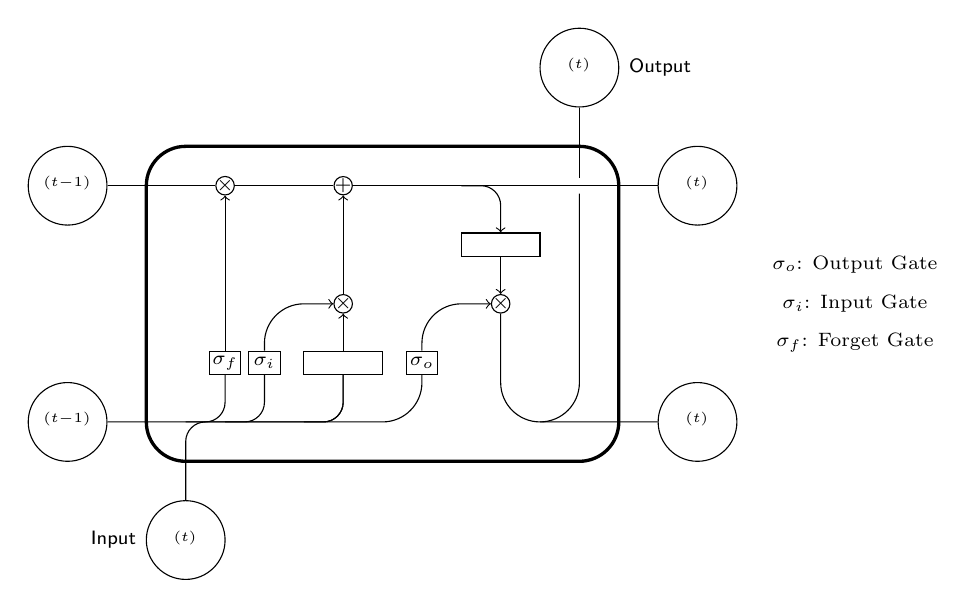
\begin{tikzpicture}[
    % GLOBAL CFG
    font= \scriptsize,
    %>=LaTeX,
    % Styles
    cell/.style={% For the main box
        rectangle,
        rounded corners=5mm,
        draw,
        very thick,
        },
    operator/.style={%For operators like +  and  x
        circle,
        draw,
        inner sep=-0.5pt,
        minimum height =.2cm,
        },
    function/.style={%For functions
        ellipse,
        draw,
        inner sep=1pt
        },
    ct/.style={% For external inputs and outputs
        circle,
        draw,
        %line width = .75pt,
        minimum width=1cm,
        inner sep=1pt,
        },
    gt/.style={% For internal inputs
        rectangle,
        draw,
        minimum width=4mm,
        minimum height=3mm,
        inner sep=1pt
        },
    mylabel/.style={% something new that I have learned
        font=\scriptsize\sffamily
        },
    ArrowC1/.style={% Arrows with rounded corners
        rounded corners=.25cm,
        %thick,
        },
    ArrowC2/.style={% Arrows with big rounded corners
        rounded corners=.5cm,
        %thick,
        },
    ]

%Start drawing the thing...
    % Draw the cell:
    \node [cell, minimum height =4cm, minimum width=6cm] at (0,0){} ;

    % Draw inputs named ibox#
    \node [gt] (ibox1) at (-2,-0.75) {$\sigma_f$};
    % forget
    \node [gt] (ibox2) at (-1.5,-0.75) {$\sigma_i$};
    % input
    \node [gt, minimum width=1cm] (ibox3) at (-0.5,-0.75) {$\tahn$};
    \node [gt] (ibox4) at (0.5,-0.75) {$\sigma_o$};
    % output

   % Draw opérators   named mux# , add# and func#
    \node [operator] (mux1) at (-2,1.5) {$\times$};
    \node [operator] (add1) at (-0.5,1.5) {+};
    \node [operator] (mux2) at (-0.5,0) {$\times$};
    \node [operator] (mux3) at (1.5,0) {$\times$};
    \node [gt, minimum width=1cm] (func1) at (1.5,0.75) {$\tahn$};
    % memory cell

    % Draw External inputs? named as basis c,h,x
    \node[ct, label={[mylabel]}] (c) at (-4,1.5) {$\cb^{(t-1)}$};
    \node[ct, label={[mylabel]}] (h) at (-4,-1.5) {$\h^{(t-1)}$};
    \node[ct, label={[mylabel]left:Input}] (x) at (-2.5,-3) {$\x^{(t)}$};

    % Draw External outputs? named as basis c2,h2,x2
    \node[ct, label={[mylabel]}] (c2) at (4,1.5) {$\cb^{(t)}$};
    \node[ct, label={[mylabel]}] (h2) at (4,-1.5) {$\h^{(t)}$};
    \node[ct, label={[mylabel]right:Output}] (x2) at (2.5,3) {$\h^{(t)}$};

    \node (fg) at (6,-0.5) {$\sigma_f$: Forget Gate};
    \node (ig) at (6,0) {$\sigma_i$: Input Gate};
    \node (og) at (6,0.5) {$\sigma_o$: Output Gate};

% Start connecting all.
    %Intersections and displacements are used.
    % Drawing arrows
    \draw [ArrowC1] (c) -- (mux1) -- (add1) -- (c2);

    % Inputs
    \draw [ArrowC2] (h) -| (ibox4);
    \draw [ArrowC1] (h -| ibox1)++(-0.5,0) -| (ibox1);
    \draw [ArrowC1] (h -| ibox2)++(-0.5,0) -| (ibox2);
    \draw [ArrowC1] (h -| ibox3)++(-0.5,0) -| (ibox3);
    \draw [ArrowC1] (x) -- (x |- h)-| (ibox3);

    % Internal
    \draw [->, ArrowC2] (ibox1) -- (mux1);
    \draw [->, ArrowC2] (ibox2) |- (mux2);
    \draw [->, ArrowC2] (ibox3) -- (mux2);
    \draw [->, ArrowC2] (ibox4) |- (mux3);
    \draw [->, ArrowC2] (mux2) -- (add1);
    \draw [->, ArrowC1] (add1 -| func1)++(-0.5,0) -| (func1);
    \draw [->, ArrowC2] (func1) -- (mux3);

    %Outputs
    \draw [-, ArrowC2] (mux3) |- (h2);
    \draw (c2 -| x2) ++(0,-0.1) coordinate (i1);
    \draw [-, ArrowC2] (h2 -| x2)++(-0.5,0) -| (i1);
    \draw [-, ArrowC2] (i1)++(0,0.2) -- (x2);
\end{tikzpicture}
}

    \caption[Long short term memoory cell]{%
        Long short term memory cell, merged lines stack vectors, split lines duplicate
        vector~\citep{goodfellow_deep_2016,yu_review_2019}\label{fig:lstm}
    }
\end{figure}
The \ac{LSTM} also improves upon the vanishing gradients problem associated with
increasingly deep \acp{NN}~\citep{sherstinsky_fundamentals_2020}
The clipping gradients technique is often used to help with exploding
gradients~\citep{goodfellow_deep_2016}.
A so-called cell is shown in Figure~\ref{fig:lstm}.
It shows the basic structure, representing the recurrent building block of
\acp{LSTM}~\citep{goodfellow_deep_2016}.
The three gates (input, forget, output) help make the \ac{LSTM} a widely used \ac{NN} model.
The gates calculate weights between 0 and 1 (thus the use of $\sigma$) used to control
the flow of information~\citep{goodfellow_deep_2016}.
The forget gate is part of a self-loop which helps to accumulate information longer, the input
gate helps to focus on the relevant characteristics of the input information,
and the output gate removes irrelevant information for the output and the next
cell~\citep{goodfellow_deep_2016}.
\begin{equation}\label{eq:lstm-gates}
    \begin{pmatrix}
        \textbf{i}_t \\
        \textbf{f}_t \\
        \textbf{o}_t \\
        \textbf{g}_t
    \end{pmatrix}
    =
    \begin{pmatrix}
        \sigma \\
        \sigma \\
        \sigma \\
        \tahn
    \end{pmatrix}
    T
    \begin{pmatrix}
        \x_{t} \\
        \h_{t-1}
    \end{pmatrix}
\end{equation}
\begin{equation}\label{eq:lstm-c}
    \textbf{c}_t=\textbf{f}_t\otimes\textbf{c}_{t-1} + \textbf{i}_t\otimes\textbf{g}_t
\end{equation}
\begin{equation}\label{eq:lstm-h}
    \h_t=\textbf{o}_t\otimes\tahn(\textbf{c}_t)
\end{equation}
Equations~\ref{eq:lstm-gates},~\ref{eq:lstm-c}, and~\ref{eq:lstm-h} show the calculations
performed for a single timestep~\citep{xu_show_2016}.
$\sigma$ and $\tahn$ denote the application of activation functions after the weight matrix $T$
is multiplied by the stacked input $\x_t,\h_{t-1}$~\citep{zaremba_recurrent_2015}.
$\textbf{i}_t,\textbf{f}_t,\textbf{o}_t$ are the output of the input gate, forget gate, and output
gate.
$\textbf{c}_t,\textbf{h}_t$ are the cell states and outputs to the next step or the
prediction sequence~\citep{zaremba_recurrent_2015}.

\acp{RNN} are often used with the \ac{EnDe} mechanism introduced by~\cite{cho_learning_2014}.
This mechanism is a structure for \ac{NN} that is used for various problems.
Initially, it was designed to use \acp{RNN} to transform an input sequence into an output sequence,
e.g., translation~\citep{cho_learning_2014}.
The output of which can be of variable length (a special token usually indicates the
end)~\citep{cho_learning_2014,asadi_encoder-decoder_2020}.
The \ac{EnDe} mechanism entails two parts: The encoder, which transforms the input into a
different representation, compresses all the information from the input into a feature vector;
the decoder uses the extracted features to generate the output
predictions~\citep{asadi_encoder-decoder_2020,cho_learning_2014}.
The decoder can thus use the whole input context at once~\citep{asadi_encoder-decoder_2020}.
The output associated with decoders is sequential~\citep{asadi_encoder-decoder_2020}.
The mechanism can be implemented in different ways.
Both purely \acp{RNN} based~\citep{cho_learning_2014} implementations and mixtures along with
\acp{CNN}~\citep{ghosh_visual_2017} exist~\citep{asadi_encoder-decoder_2020}.
The \ac{RNN} \ac{EnDe} can transform a sequence of variable lengths into another
sequence with different variable lengths~\citep{cho_learning_2014}.
The encoder processes the input sequence and crafts a representation vector that encodes information
and context for the whole input sequence, which can then be used for every step in the decoder
network (see Figure~\ref{fig:enc-dec-rnn})~\citep{cho_learning_2014}.
\begin{figure}[h]
    \centering
    \resizebox{0.8\linewidth}{!}{\scriptsize%
\begin{tikzpicture}[%
    hid/.style 2 args={%
        rectangle split,
        rectangle split horizontal,
        draw=#2,
        rectangle split parts=#1,
        fill=#2!20,
        outer sep=1mm
    }
]
    % draw input nodes
    \foreach \i [count=\step from 1] in {the,blue,house,{{$<$bos$>$}}}
    \node (i\step) at (2*\step, -2) {\i};
    % draw output nodes
    \foreach \t [count=\step from 4] in {das,blaue,Haus,{{$<$eos$>$}}} {
        \node[align=center] (o\step) at (2*\step, +2.75) {\t};
    }
    % draw embedding and hidden layers for text input
    \foreach \step in {1,...,3} {
        \node[hid={3}{red}] (h\step) at (2*\step, 0) {};
        \node[hid={3}{red}] (e\step) at (2*\step, -1) {};
        \draw[->] (i\step.north) -> (e\step.south);
        \draw[->] (e\step.north) -> (h\step.south);
    }
    % draw embedding and hidden layers for label input
    \foreach \step in {4,...,7} {
        \node[hid={3}{yellow}] (s\step) at (2*\step, 1.25) {};
        \node[hid={3}{blue}] (h\step) at (2*\step, 0) {};
        \node[hid={3}{blue}] (e\step) at (2*\step, -1) {};
        \draw[->] (e\step.north) -> (h\step.south);
        \draw[->] (h\step.north) -> (s\step.south);
        \draw[->] (s\step.north) -> (o\step.south);
    }
    \draw[->] (h3.east) edge[->,out=330,in=200] (h5.south);
    \draw[->] (h3.east) edge[->,out=330,in=190] (h6.south);
    \draw[->] (h3.east) edge[->,out=330,in=180] (h7.south);
    % edge case: draw edge for special input token
    \draw[->] (i4.north) -> (e4.south);
    % draw recurrent links
    \foreach \step in {1,...,6} {
        \pgfmathtruncatemacro{\next}{add(\step,1)}
        \draw[->] (h\step.east) -> (h\next.west);
    }
    % draw predicted-labels-as-inputs links
    \foreach \step in {4,...,6} {
        \pgfmathtruncatemacro{\next}{add(\step,1)}
        \path (o\step.north) edge[->,out=45,in=225] (e\next.south);
    }
\end{tikzpicture}
}
%
    \caption[Sequence to sequence encoder decoder architecture]{%
        Sequence to sequence encoder decoder
        architecture~\citep{cho_learning_2014}\label{fig:enc-dec-rnn}
    }
\end{figure}
An example used for an \ac{EnDe} architecture with a \ac{CNN} encoder and a \ac{RNN} decoder
would be image captioning~\citep{asadi_encoder-decoder_2020}.
The image is encoded into a vector which includes context for the whole
image~\citep{asadi_encoder-decoder_2020}.
\begin{figure}[h]
    \centering
    \resizebox{0.55\linewidth}{!}{\scriptsize%
\begin{tikzpicture}[%
    item/.style={circle,draw,align=center,minimum width=1.5cm},
    itemc/.style={item,on chain,join},scale=0.5,
]
    \node[rectangle,minimum size=1.5cm,draw=black] (At+1) {CNN};

    \node[right=2em of At+1,rectangle,draw=black] (feat) {Feture Vector};


    \node[right=2em of feat,item] (Bt-1) {$\h^{(1)}$};
    \node[right=2em of Bt-1,item] (Bt) {$\h^{(2)}$};
    \node[right=2em of Bt,item] (Bt+1) {$\h^{(3)}$};

    \draw[->] (Bt-1) -- (Bt)
        node[midway,above] (W) {};
    \draw[->] (Bt) -- (Bt+1)
        node[midway,above] (W) {};
    \draw[->,dashed] (Bt+1) -- ++(+2,0) node[right] (end) {};

    \draw[->] (Bt-1.north) -- ++ (0,2em) node[above,item] (h1) {$\hat{\y}^{(1)}$};
    \draw[->] (Bt.north) -- ++ (0,2em) node[above,item] (h2) {$\hat{\y}^{(2)}$};
    \draw[->] (Bt+1.north) -- ++ (0,2em) node[above,item] (h3) {$\hat{\y}^{(3)}$};


    \draw[->] (h1) -- (Bt);
    \draw[->] (h2) -- (Bt+1);
    \draw[->,dashed] (h3) -- (end);

    \draw[->] (At+1.east) -- (feat.west);
    \draw[->] (feat.east) -- (Bt-1.west);
\end{tikzpicture}
}
%
    \caption[Image to sequence encoder decoder architecture]{%
        Image to sequence encoder decoder
        architecture~\citep{asadi_encoder-decoder_2020}\label{fig:enc-dec-cnn}
    }
\end{figure}

\section{Scene Text Spotting}\label{se:sts}
%% intro
% def, ocr vs sts
\ac{OCR} is the concept of extracting typed, handwritten, or printed text
from an image~\citep{zhao_improving_2020}.
Achieving satisfactory performance of \ac{OCR} systems in natural scenes is still
challenging~\citep{zhao_improving_2020, chen_text_2021}.
Such scenes entail natural scenes captured by a camera~\citep{chen_text_2021, baek_what_2019}.
The difficulties arise from diversity and variability of text, complexity, and interference from
backgrounds, and poor imaging conditions.
In these conditions, \ac{OCR} is known as \ac{STS}~\citep{long_scene_2021}.
% DL influence
Before the advent of \ac{DL}, researchers in the field had to hand-craft
features~\citep{long_scene_2021}.
\ac{DL} automates the feature generation process with its representation and learning
capabilities~\citep{long_scene_2021,goodfellow_deep_2016}.
Because of this, \ac{DL} methods are the preferred tools for performing
\ac{STS}~\citep{long_scene_2021}.
% STD, STR, end to end
\ac{OCR} and \ac{STS} are often divided into two subcategories (Scene) Text Detection and (Scene)
Text Recognition~\citep{zhao_improving_2020, long_scene_2021,chen_text_2021}.
For \ac{STD}, the task is to localize text instances in the image, whereas the \ac{STR} task
is to recognize/categorize text from already cropped images~\citep{chen_text_2021}.
Note that a system that performs both \ac{STR} and \ac{STD} in one continuous pipeline is called
an end-to-end approach~\citep{chen_text_2021}.

%% evaluation metrics
% XXX: properties and pros for different metrics
% XXX: table with task, metric, properties/why it's used
The right evaluation metrics must be used to assess the performance of developed approaches.
% STD
The popular protocols Precision, Recall, and the \fone\ are used to compare
approaches for \ac{STD}~\citep{long_scene_2021}.
The metrics are derived with values from the confusion matrix (see
Tabel~\ref{tb:confusionMatrix})~\citep{davis_relationship_2006}.
\begin{table}[ht]
    \centering\scriptsize
    \makebox[\textwidth][c]{\begin{tabular}{cccc}
        \toprule
                  & & \multicolumn{2}{c}{\textbf{Ground Truth}} \\
                  & & positive & negative \\
        \midrule
            \textbf{Prediction} & \multicolumn{1}{c|}{\makecell{positive\\negative}}
                            & \makecell{True Positive \\ False Negative }
                            & \makecell{False Positive \\ True Negative} \\
        \bottomrule
    \end{tabular}}
    \caption{Confusion Matrix\label{tb:confusionMatrix}}
\end{table}
\begin{equation}\label{eq:P}
    \text{Precision}=\frac{\text{True Positive}}{\text{True Positive + False Positive}}
\end{equation}
\begin{equation}\label{eq:R}
    \text{Recall}=\frac{\text{True Positive}}{\text{True Positive + False Negative}}
\end{equation}
\begin{equation}\label{eq:f1}
    F_1\text{-Score}=\frac{2\cdot \text{Precision}\cdot \text{Recall}}{\text{Precision}+\text{Recall}}
\end{equation}
The difference of metrics for the task manifests itself in the way the values of the confusion matrix
are calculated~\citep{long_scene_2021}.
Note that the tradeoff between False Positives and Fales Negatives manifests itself in the
Precision-versus-Recall curve~\citep{su_relationship_2015}.
\fone\ is also referred to as the harmonic mean (between Precision and
Recall)~\citep{he_icpr2018_2018}.
% XXX: PvR curve figure
% XXX: introduce ROC curve --- ratio of true positive rate and false positive rate, and
%           relationship to PvR curve/AP
\ac{STD} differs mainly in how the protocols match the prediction to the ground
truth~\citep{long_scene_2021}.
Detectors have multiple predictors which regress the placing and sizing of \acp{BB}.
More information on this will follow in Chapter~\ref{ch:research}.
Matching is the process of assigning a \ac{BB} prediction to the ground
truth, e.g.,~\cite{liu_ssd_2016,liao_textboxes_2018}.
The PASCAL approach defines the \ac{IOU} (see Equation~\ref{eq:iou}).
\begin{equation}\label{eq:iou}
    \ac{IOU}=
            \frac{\text{area of intersection between truth and prediction}}{\text{area of union
            between truth and prediction}}
\end{equation}
For PASCAL, the prediction will be matched if the \ac{IOU} value is larger than a
threshold~\citep{long_scene_2021}.
A match is considered a True Positive, the other values are assigned
accordingly~\citep{sun_icdar_2019}.
% more BB have IOU>threshold -> depending on situation all or greatest value
Other evaluation approaches are mostly based on \ac{IOU}, e.g., MSRA-TD 500 evaluates the rotation
from the \ac{BB} compared to the truth and the \ac{IOU}
threshold~\citep{long_scene_2021}.
\cite{long_scene_2021} argues that researchers in the field of \ac{STD} should consider \ac{AP}
as the primary evaluation protocol rather than \fone.
According to~\cite{su_relationship_2015}, \ac{AP} can be considered the area under the
Precision-versus-Recall curve.
\fone, on the other hand, only considers singular instances on that curve~\citep{long_scene_2021} and
is sensitive to the tradeoff, while \ac{AP} is invariant to it~\citep{shi_icdar2017_2017}.

% STR
For \ac{STR}, the evaluation can be based on character-level or word-level.
There is no need to match ground truth to prediction, as the image is already
cropped~\citep{long_scene_2021}.
Often lexicons that contain possible words are used by \ac{STR}.
Testing and real-world performance can depend strongly on these
lexicons~\citep{chen_text_2021,long_scene_2021}.
The equations~\ref{eq:wordRecognitionAccuracy} and~\ref{eq:wordErrorRate} show metrics based on
word-level~\citep{chen_text_2021}.
\begin{equation}\label{eq:wordRecognitionAccuracy}
\text{Word Recognition Accuracy} = \frac{\text{correctly recognized words}}{\text{total words}}
\end{equation}
\begin{equation}\label{eq:wordErrorRate}
    \text{Word Error Rate} = 1 - \text{Word Recognition Accuracy}
\end{equation}
An example for a character-based metric would be $1 - $NED, where \ac{NED}
calculates the distance between prediction and ground truth (see Equation~\ref{eq:ned}).
\begin{equation}\label{eq:ned}
    \text{NED} = \frac{1}{N}\sum_{i=1}^N \frac{D(s_i,\hat{s}_i)}{\max(l_i,\hat{l_i})}
\end{equation}
D denotes the Levenshtein distance, s denotes the text, l denotes the text length, and N is the total
number of text lines~\citep{shi_icdar2017_2017}.
For \ac{STR}, \ac{NED} is used over the whole dataset~\citep{karatzas_icdar_2013}.

\ac{STS} is oriented to both \ac{STD} and \ac{STR}.
The prediction must be matched to the ground truth, like for \ac{STD}~\citep{long_scene_2021}.
For comparing predictions and matching the respective ground truths that have been matched, \ac{NED}
is used~\citep{chen_text_2021}.
For end-to-end recognition~\citep{karatzas_icdar_2013,karatzas_icdar_2015}, the primary evaluation
protocols that are used include Precision, Recall, \fone, and \ac{AED}~\citep{chen_text_2021}.
A sample is considered a True positive if the \ac{NED} distance between predictions and
matched ground truths equals 0~\citep{sun_icdar_2019} (one sample can have multiple text
instances).
\ac{AED} is the sum of \ac{NED} values divided by the number of pictures~\citep{chen_text_2021}.
Note that competitions often define their variants of the metrics,
e.g.,~\cite{he_icpr2018_2018,shi_icdar2017_2017}.
Case sensitivity and matching criteria are examples of changing properties of metrics.

To compare approaches with these metrics, benchmark datasets that have different characteristics
are used.
\begin{table}[ht]
    \centering\scriptsize
    \begin{tabular}{p{.25\textwidth}p{.05\textwidth}p{.05\textwidth}p{.15\textwidth}p{.25\textwidth}}
        \textbf{Dataset (year)}&\textbf{\ac{STD}}&\textbf{\ac{STR}}&\textbf{Text Orientation}
                                                            &\textbf{Characteristics} \\
        \toprule
        ICDAR (2013) & \checkmark& \checkmark&Horizontal& --- \\
        IIIT 5K-Word (2012) & &\checkmark&Horizontal& Cropped, variance in font, color, size and
                                                        noise~\citep{long_scene_2021} \\
        ICDAR (2015) & \checkmark& \checkmark&Multi-oriented& Low resolution, small text
                                                                instances~\citep{liao_mask_2020} \\
        MSRA-TD500 (2012) & \checkmark&&Multi-Oriented& Extreme aspect ratios~\citep{liao_mask_2020}\\
        ICDAR MLT (2017) & \checkmark&\checkmark&Curved& Multilingual~\citep{long_scene_2021}  \\
        SCUT CTW1500 (2017)& \checkmark& &Curved& --- \\
        Total-Text (2017) & \checkmark& \checkmark&Curved& --- \\
        \bottomrule
    \end{tabular}
    \caption{Benchmark datasets and their properties\label{tb:datasets}}
\end{table}
Table~\ref{tb:datasets} lists a couple of influential benchmark datasets and their fundamental
properties.
ICDAR (2013) references the Focused Scene Text dataset~\citep{karatzas_icdar_2013} and ICDAR 2015
to the Incidental Text Competition dataset~\citep{karatzas_icdar_2015}.
The second and third columns indicate whether the dataset provides annotations for the tasks.
The Text Orientation column specifies the most complicated orientation present in the dataset
(Curved $\subset$ Multi-oriented $\subset$ Horizontal).
A collection of images that shows representative examples taken out of benchmark datasets can
be found in Appendix~\ref{ch:app-datasets}.
